% Chapter Template

\section{Data Sources}
We use two data sources for the model. To calibrate the agent based model we use data obtained from Eurostat. For the household sector we use data which is obtained from the Statistics Netherlands Microdata database\footnote{At https://www.cbs.nl/en-gb/onze-diensten/customised-services-microdata/microdata-conducting-your-own-research more information can be found about this database.}. The Microdata database consists out of linkable data at the level of individuals, companies and addresses. The model is calibrated for each period $t$ where the periods are set to be quarters. In principle, each agent represents a natural or legal entity such as households, firms, government entities or other institutions from the Netherlands. However, due to data privacy regulation which prevent the Statistics Netherlands Microdata database from leaving internal systems, we have opted to summarize the Microdata by using multivariate empirical distributions which are allowed to leave internal systems. The Netherlands is a small open economy with 18 million inhabitants\footnote{Data is retrieved from the Statistics Netherlands website https://opendata.cbs.nl/\#/CBS/en/ accessed at March 22nd 2023.}. The social system of the Netherlands is well developed and consequently government expenditures amounted to 44.5\% of GDP. The Netherlands trades extensively with export amounting to 51\% of GDP whereas import amounts to 45\% of GDP. The Netherlands moreover has a labour income share of 77.3\%.

The model is calibrated like \cite{poledna_economic_2019}. The parameters are calibrated using the Statistics Netherlands Microdata database, census and business demography, and input-output tables, government statistics and sector accounts, and national accounts. The source of the data for each parameter is reported in table \ref{tab:tables_main}.  

\begin{table}[!htb]
	\caption{Eurostat data tables} \label{tab:tables_main}
	\centering
	\resizebox{.88\columnwidth}{!}{
	\begin{tabular}{ll}
		\toprule
		Name & Code \\
		\midrule
		Population by current activity status, NACE Rev. 2 activity and NUTS 2 region & cens\_11an\_r2 \\
		Business demography by legal form (from 2004 onwards, NACE Rev. 2)	&	bd\_9ac\_l\_form\_r2 \\
		Symmetric input-output table at basic prices (product by product)	&	naio\_10\_cp1700 \\
		Cross-classification of fixed assets by industry and by asset (stocks)	&	nama\_10\_nfa\_st \\
		Government revenue, expenditure and main aggregates	&	gov\_10a\_main \\
		General government expenditure by function (COFOG)	& gov\_10a\_exp	\\
		Quarterly non-financial accounts for general government & gov\_10q\_ggnfa \\
		Quarterly government debt & gov\_10q\_ggdebt \\
		Financial balance sheets	&	nasq\_10\_f\_bs \\
		Non-financial transactions (annually)	&	nasa\_10\_nf\_tr \\
		Non-financial transactions (quarterly) &	nasq\_10\_nf\_tr \\
		GDP and main components (output, expenditure and income) & namq\_10\_gdp \\
		Money market interest rates - quarterly data & irt\_st\_q \\
		\bottomrule
	\end{tabular}
	}
	\begin{tablenotes}
		\footnotesize \item \textit{Note}: The codes under which the respective datasets are available from Eurostat (such as, e.g. naio\_10\_cp1750) are shown in the second column.
	\end{tablenotes}
\end{table}
\subsection{Census and Demography Data}
The parameters which specify the number of agents are directly related to census and business demography data.  We used database ‘‘Population by current activity status, NACE Rev. 2 activity and NUTS 2 region’’ (cens\_11an\_r2) to calibrate  to the number of active persons $H^{\text{act}}$ in the Netherlands in 2011. Contrary to \cite{poledna_economic_2019}, we scale the model to 1:2000 due to computational and privacy legislative limitations. This gives us 5891 households and 780 firms. See table \ref{tab:parameter_overview} for an overview of the parameters. The classification of industries is done using the statistical classification of economic activities in the European Community (NACE). For the European Union Eurostat has compiled  tables including input–output tables, demographic data, and cross-classification tables with a breakdown of 64 activities/products. We exclude the sectors ‘‘Services of households as employers and services produced by households for own use’’ (T) and ‘‘Services provided by extraterritorial organizations and bodies’’ (U ) in the model, as these have zero output in the Netherlands. Consequently, we set the number of industries (S) and the number of products (G) to 62. Business demography data (bd\_9ac\_l\_form\_r2) is used to set the parameters concerned with the number of firms for each industry $I_s$. Similar to \cite{poledna_economic_2019} we set the number of foreign firms that import domestic goods to 50\% and the number of government entities to 25\% which corresponds to to the share of exports of total value added and total share of government consumption in total value added respectively.
The classification of industries is done using the statistical classification of economic activities in the European Community (NACE). For the European Union Eurostat has compiled  tables including input–output tables, demographic data, and cross-classification tables with a breakdown of 64 activities/products.
\subsection{Input-output tables}
The parameters which are related to productivity and technology, capital formation and consumption are calculated from the input-output tables. The parameters vary over the industries and are calibrated once every year meaning that they do not change over the quarters of a year. To calibrate the technology, consumption and capital formation coefficients
$(a_{sg}, \ b_g^{CF}, \ b_g^{HH}, \ b_g^{CFH}, \ c_g^G, \ c_g^E,\text{ and }c_g^I)$ and the productivity coefficient of intermediate inputs and nex tax rates $(\beta_i, \tau_i^Y, \text{ and } \tau_i^K)$ we use the symmetric input–output table at basic prices (industry by industry) (naio\_10\_cp1750). Some parameters are calibrated using both national accounting data and input-output tables. The parameters are calculated by normalizing the tables column wise.\\

Some parameters use both data from input-output tables, structural business statistics, and sectoral accounts. We can combine the data of these sources by using cross-classification tables. The parameters of productivity coefficients for labour and capital $(\overline{\alpha}_i, \ \kappa_i)$, the depreciation rate $(\delta_i)$, and the average wage rate are calibrated $(\overline{w}_i)$ in this way.
\begin{figure}
    \centering
    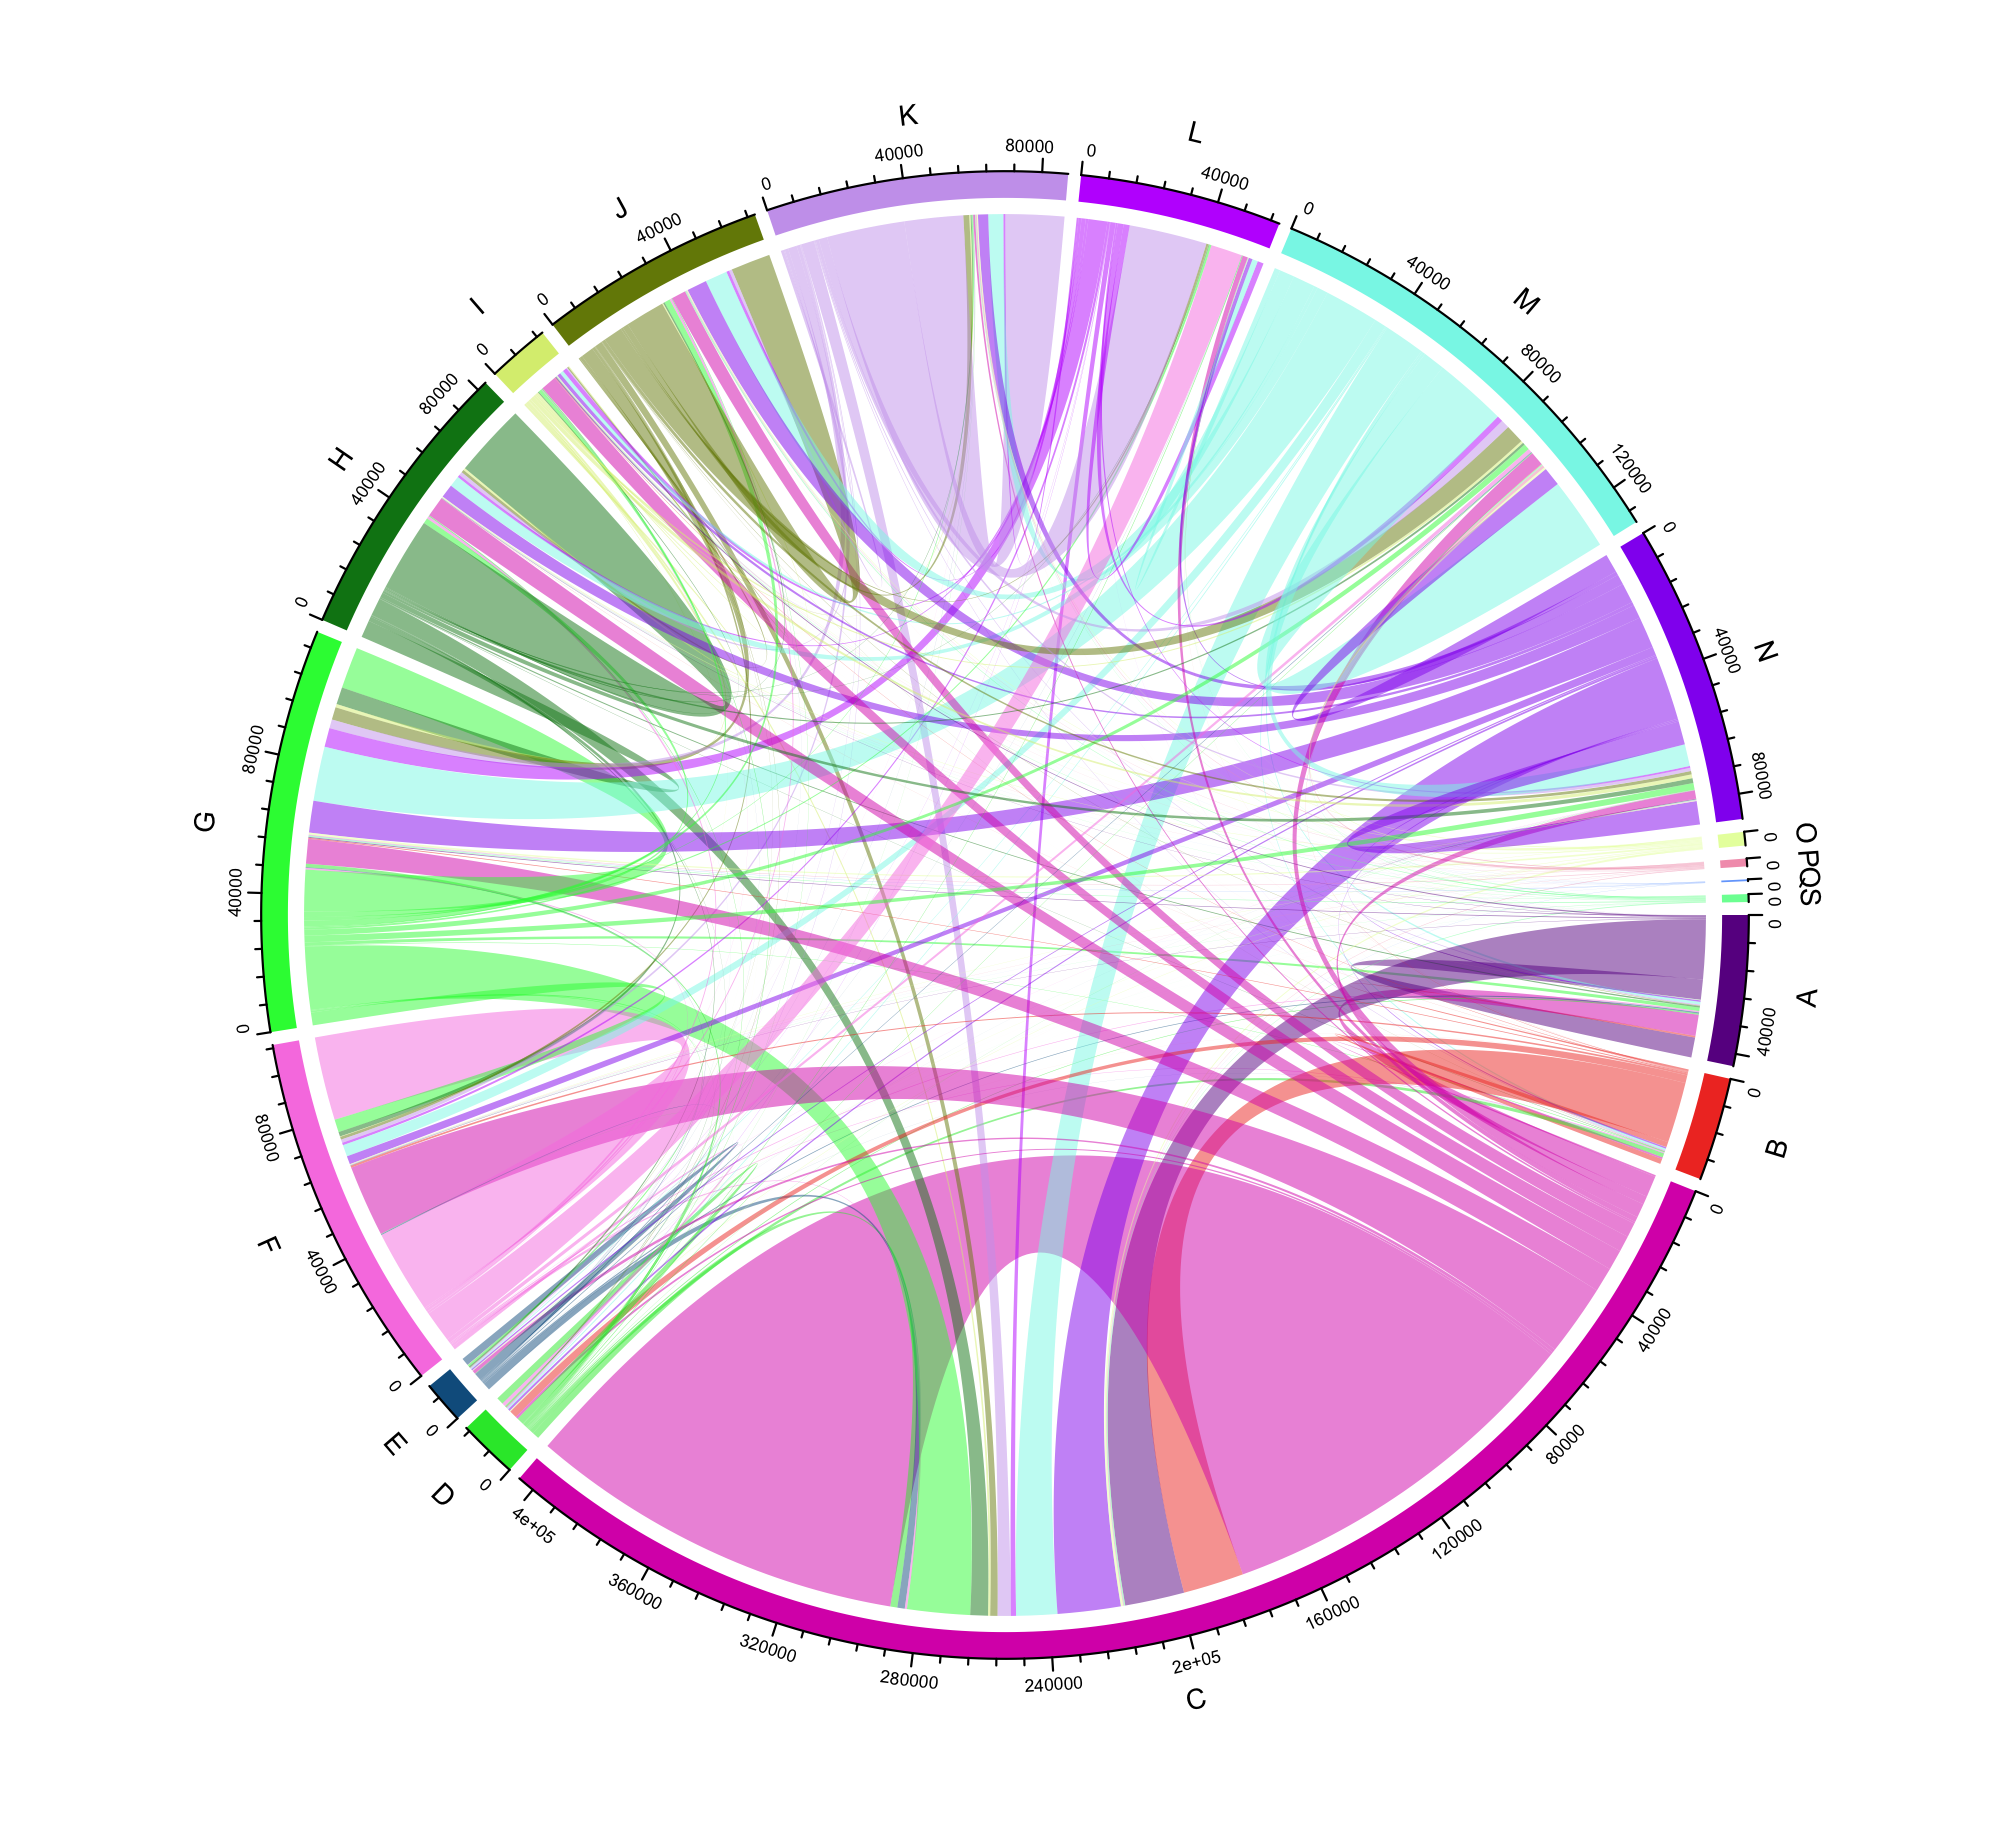
\includegraphics[trim = 3cm 3cm 3cm 3cm, clip, width = \textwidth]{figs/Rplot03.png}
    \captionsetup{singlelinecheck=off}
    \caption[foo bar]{Intermediate consumption between 19 industries derived from Eurostat input-output table.\\[-25pt]
       \begin{multicols}{3}
            \begin{itemize}[leftmargin=*, noitemsep, topsep=0pt]
            \tiny
              \item[A] Agriculture, forestry and fishing
              \item[B] Mining and quarrying
              \item[C] Manufacturing
              \item[D] Electricity, gas, steam and air conditioning supply
              \item[E] Water supply
              \item[F] Construction
              \item[G] Wholesale and retail trade
              \item[H] Transportation and storage
              \item[I] Accommodation and food service activities
              \item[J] Information and communication
              \item[K] Financial and insurance activities
              \item[L] Real estate activities
              \item[M] Professional, scientific and technical activities
              \item[N] Administrative activities
              \item[O] Public administration and defense, compulsory social security
              \item[P] Education
              \item[Q] Human health and social work activities
              \item[R] Arts, entertainment and recreation
              \item[S] Other services activities
            \end{itemize}
        \end{multicols}
    }
    \label{fig:IO}
\end{figure}
\subsection{Government Statistics and Sector Accounts}
We use national accounting identities to calculate the tax rates. The tax rates are calculated in such a way that rates they match the financial flows observed in input–output tables, government statistics, and sector accounts. An average tax rate for an institutional sector (firms, households, etc.) are defined as the aggregate tax flow of divided by the aggregate monetary flow that is the base of the tax. These tax rates are computed per calendar year due to data availability. Moreover, the same tax rate is applied to every individual agent\footnote{The Netherlands has a progressive marginal tax system which we refrain from for model parsimony.}. The firm profit tax rate ($\tau^{\text{FIRM}}$) is equal to the ratio of total corporate tax flows to total operating surplus and mixed income, which we take from sector accounts (non-financial transactions (nasa\_10\_nf\_tr)) and from input–output tables respectively. The rates for social security contributions both for employers ($\tau^{\text{SIF}}$) and employees ($\tau^{\text{SIW}}$) are calibrated similarly using input–output tables and government statistics. The input–output tables are used to calibrated the value added tax rates ($\tau^{\text{VAT}}$,$\tau^{\text{CF}}$, $\tau^{\text{G}}$, $\tau^{\text{EXPORT}}$).\\

Firms’ dividend payout ratio ($\theta^{\text{DIV}}$) is equal to interest and dividend receipts plus mixed income by the household sector in the sector accounts (non-financial transactions (nasa\_10\_nf\_tr)) divided by total net operating surplus and mixed income as obtained from input–output tables. We use the sector accounts to obtain the risk premium ($\mu$) paid on firms’ outstanding debt and it is calculated such that total interest payments in our model financial market, where firm debt constitutes the only financial asset held by the banking sector, matches empirically observed interest payments paid by non-financial and financial corporations in the sector accounts (non-financial transactions (nasq\_10\_nf\_tr)). We calculate the risk premium ($\mu$) as the difference between the 3-month Euribor interest rate obtained from money market interest rates (irt\_st\_q) and the observed interest payments divided by the liabilities of non-financial corporations, which is obtained from sector accounts (financial balance sheets (nasq\_10\_f\_bs)). Finally, the interest rate on government debt ($r^G$) is calibrated to the interest due per quarter by the general government as a proportion of the total government debt which is obtained from government statistics (gov\_10q\_ggdebt, gov\_10q\_ggnfa).
\subsection{Statutory guidelines, financial regulations (Basel III), and banking practices}
We also calibrate some parameters according to statutory guidelines, financial regulation (Basel III), and banking practices. The capital ration $(\zeta)$ is set according to Basel III financial regulations. The central bank inflation target $(\pi^*)$ is set to 2\% according to the statutes of the ECB. The rate of debt instalment $(\theta)$ is set to 5\% which means that firms pay 5\% of their total outstanding debt each quarter. The maximum allowed loan-to-value ratio of banks $(\zeta^{\text{LTV}})$ is set to 60\%. New firms' loan-to-value ratio $(\zeta^{\text{b}})$ which replace bankrupt firms are set to 50\%. 
\subsection{Exogeneously estimated from national accounts and money market interest rates}
We use the national accounts (namq\_10\_gdp) and the money market interest rates (irt\_st\_q) to estimate exogenous processes such as imports, exports, final consumption expenditure of the general government, inflation and GDP growth of the euro area. These are estimated from the data of the first quarter of 1997 to the quarter of calibration.

\begin{table}[!htbp]
	\caption{Model parameters} \label{tab:parameter_overview}
	\centering
	\resizebox{.83\columnwidth}{!}{
	% \begin{ruledtabular}
		\begin{tabular}{llrl}
			\toprule
			Parameter & Description & Value & Source\\
			\midrule
			$G$/$S$ & Number of products/industries & 62 & \multirow{6}{*}{\rotatebox[origin=c]{90}{\parbox[c]{2.25cm}{\centering census data, business demography data}}} \\ 
			$H^{\mathrm{act}}$ & Number of economically active persons & 7860391 & \\ 
			$H^{\mathrm{inact}}$ & Number of economically inactive persons & 3921200 & \\ 
			$J$ & Number of government entities & 152820 & \\ 
			$L$ & Number of foreign consumers & 305639 & \\ 
			$I$ & Number of firms& 1536974  & \\ 
			\midrule
            $\beta$ & Household discount rate&  0.9276 &  \multirow{4}{*}{\rotatebox[origin=c]{90}{\parbox[c]{1.5cm}{\centering CBS Micro-data}}} \\ 
			$1/\sigma$ & Intertemporal elasticity of substitution  & 0.013 & \\ 
            $x_0$ & Size of transaction cost of investment&  0.1 & \\ 
            $x_1$& Convexity of transaction cost of investment &  1.5 & \\ 
            \midrule
			$\bar{\alpha}_{i}$ & Average productivity of labour of the $i$\textsuperscript{th} firm & \multirow{14}{*}{\rotatebox[origin=c]{90}{\parbox[c]{5cm}{\centering parameters are firm/sector specific; see table \ref{table:sector_parameters}}}} & \multirow{14}{*}{\rotatebox[origin=c]{90}{\parbox[c]{5cm}{\centering input-output tables}}} \\ 
			$\kappa_{i}$ & Productivity of capital of the $i$\textsuperscript{th} firm & & \\ 
			$\beta_{i}$ & Productivity of intermediate consumption of the $i$\textsuperscript{th} firm & & \\ 
			$\delta_{i}$ & Depreciation rate for capital of the $i$\textsuperscript{th} firm & & \\ 
			$\bar{w}_{i}$ & Average wage rate of firm $i$ & & \\ 
			$a_{sg}$ & Technology coefficient of the $g$\textsuperscript{th} product in the $s$\textsuperscript{th} industry & & \\ 
			$b^{\mathrm{CF}}_g$ & Capital formation coefficient of the $g$\textsuperscript{th} product (firm investment) & & \\ 
			$b^{\mathrm{CFH}}_{g}$ & Household investment coefficient of the $g$\textsuperscript{th} product & & \\ 
			$b^{\mathrm{HH}}_{g}$ & Consumption coefficient of the $g$\textsuperscript{th} product of households & & \\ 
			$c^{\mathrm{G}}_g$ & Consumption of the $g$\textsuperscript{th} product of the government in mln. Euro & & \\ 
			$c^{\mathrm{E}}_g$ & Exports of the $g$\textsuperscript{th} product in mln. Euro & & \\ 
			$c^{\mathrm{I}}_g$ & Imports of the $g$\textsuperscript{th} product in mln. Euro & & \\ 
			$\tau^{\mathrm{Y}}_{i}$ & Net tax rate on products of the $i$\textsuperscript{th} firm & & \\ 
			$\tau^{\mathrm{K}}_{i}$ & Net tax rate on production of the $i$\textsuperscript{th} firm & & \\ 
			\midrule
			$\tau^{\mathrm{INC}}$ & Income tax rate & 0.1715 & \multirow{13}{*}{\rotatebox[origin=c]{90}{\parbox[c]{4cm}{\centering government statistics, sector accounts}}} \\ 
			$\tau^{\mathrm{FIRM}}$ & Corporate tax rate & 0.0805 & \\ 
			$\tau^{\mathrm{VAT}}$ & Value-added tax rate & 0.1381 & \\ 
			$\tau^{\mathrm{SIF}}$ & Social insurance rate (employers' contributions) & 0.2922 & \\ 
			$\tau^{\mathrm{SIW}}$ & Social insurance rate (employees' contributions) & 0.1103 & \\ 
			$\tau^{\mathrm{EXPORT}}$ & Export tax rate & 0.0024 & \\ 
			$\tau^{\mathrm{CF}}$ & Tax rate on capital formation & 0.0969 & \\ 
			$\tau^{\mathrm{G}}$ & Tax rate on government consumption & 0.0019 & \\ 
			$r^{\mathrm{G}}$ & Interest rate on government bonds & 0.0057 & \\ 
			$\mu$ & Risk premium on policy rate & 0.0243 & \\ 
			$\psi$ & Fraction of income devoted to consumption & 0.8487 & \\ 
			$\psi^{\mathrm{H}}$ & Fraction of income devoted to investment in housing & 0.0936 & \\ 
			$\theta^{\mathrm{DIV}}$ & Dividend payout ratio & 0.5354 & \\ 
			\midrule
			$\theta^{\mathrm{UB}}$ & Unemployment benefit replacement rate & 0.4054 & \multirow{6}{*}{\rotatebox[origin=c]{90}{\parbox[c]{2.5cm}{\centering Basel III, ECB statutes, banking practices, literature}}} \\
			$\theta$ & Rate of instalment on debt & 0.05 & \\ 
			$\zeta$ & Banks' capital ratio & 0.03 & \\ 
			$\zeta^{\mathrm{LTV}}$ & Loan-to-value (LTV) ratio & 0.6 & \\ 
			$\zeta^{\mathrm{b}}$ & Loan-to-capital ratio for new firms after bankruptcy & 0.5 & \\ 
			$\pi^{*}$ & Inflation target of the monetary authority & 0.005 & \\ 
			\midrule
			$\alpha^{\mathrm{G}}$ & Autoregressive coefficient for government consumption & 0.9821 & \multirow{14}{*}{\rotatebox[origin=c]{90}{\parbox[c]{5.5cm}{\centering national accounts\\ (exogenously estimated)}}} \\ 
			$\beta^{\mathrm{G}}$ & Scalar constant for government consumption & 0.1943 & \\ 
			$\sigma^{\mathrm{G}}$ & Standard deviation of government consumption & 0.0095 & \\ 
			$\alpha^{\mathrm{E}}$ & Autoregressive coefficient for exports & 0.9747 & \\ 
			$\beta^{\mathrm{E}}$ & Scalar constant for exports & 0.3029 & \\ 
			$\alpha^{\mathrm{I}}$ & Autoregressive coefficient for imports & 0.9664 & \\ 
			$\beta^{\mathrm{I}}$ & Scalar constant for imports & 0.3963 & \\ 
			$\alpha^{\mathrm{Y}^{\mathrm{EA}}}$ & Autoregressive coefficient for euro area GDP & 0.9650 & \\ 
			$\beta^{\mathrm{Y}^{\mathrm{EA}}}$ & Scalar constant for euro area GDP & 0.5152 & \\ 
			$\alpha^{\pi^{\mathrm{EA}}}$ & Autoregressive coefficient for euro area inflation & 0.3933& \\ 
			$\beta^{\pi^{\mathrm{EA}}}$ & Scalar constant for euro area inflation & 0.0024& \\ 
			$\sigma^{\pi^{\mathrm{EA}}}$ & Standard deviation of euro area inflation & 0.0023 & \\ 
			$\rho$ & Adjustment coefficient of the policy rate & 0.9287 & \\ 
			$r^{*}$ & Real equilibrium interest rate & -0.0035 & \\ 
			$\xi^{\pi}$ & Weight of the inflation target & 0.2854 & \\ 
			$\xi^{\gamma}$ & Weight of economic growth & 1.3048 & \\ 
			$C$ & Covariance matrix of euro area GDP and imports and exports & & \\ 
			\bottomrule
		\end{tabular}
	% \end{ruledtabular}
	}
	\begin{tablenotes}
		\footnotesize \item \textit{Note}: \textcolor{black}{Model parameters for the reference quarter 2014:Q1. Exogenous autoregressive coefficients and parameters of the Taylor rule are estimated over the sample 1997:Q1 to 2014:Q1. Note that the number of agents are not scaled here.}
	\end{tablenotes}
\end{table}


\subsection{Dividing Wealth between Liquid and Illiquid Assets}
We need to map the diverse household balance that is present in the CBS microdatabase to the two asset categories of liquid assets and illiquid assets. We will follow the Statistics Netherlands when dividing asset categories. We classify net liquid assets $b$ as all deposits in checking and savings accounts. Illiquid assets $k$ are defined as real estate wealth net of mortgage debt, financial assets including government bonds, corporate and private equity, and remaining properties. 
\subsection{Calibration of the Household Policy Functions}
\noindent We use the Statistics Netherlands microdata to calibrate the policy functions. We calculate the three dimensional empirical distribution of income, illiquid capital holding, and liquid capital holding for the period 2010-2019. We use this empirical distribution function to calibrate policy functions. We draw agents from the empirical distribution such that the the empirical distribution of the agents in the model match the empirical distribution. The inputs of the policy functions are either taken directly from the national accounts data, the empirical distributions, or internally defined model variables such as the return on capital $r^k_t$. \\

\noindent The aim of the calibration process of the policy functions is that the outputs of the policy function match the data we observe in the national accounts. For instance, the sum of total consumption of the agents must be as close as possible as the total consumption in the national accounts. This poses a challenge as we all the data inputs of the policy function are fixed as these are all determined by the different data sources. We have chosen to adjust the average level of consumption post hoc solving the optimal consumption model. We adjust the level of consumption until the total level of consumption matches the level of consumption seen in the national accounts. The final policy function we thus use is a adjusted version of the policy function generated by the optimal consumption problem.\\

\noindent We argue that the adjusted policy function is closer to the true policy function as the adjusted policy function matches the total level of consumption measured in the data. We have tried to match these two statistics by adjusting the parameter values by means of a general solver but this has proven to be incredibly difficult. We cannot use gradient based or surrogate optimization methods as one needs to calculate the policy function several hundred of thousands times for each calibration period. We moreover suspect that the assumptions made by the HANK model are not fully reflective of the behavioural patterns of the consumers to match the statistics given the fixed data inputs. Hence, more work is needed to find a set of assumptions such that the generated moments of the model match the empirical moments given the fixed data inputs but we leave this to future research. \footnote{For instance, the inclusion of housing wealth as a state variable and using the present bias assumption are possible extensions which \cite{laibson_present_nodate} employ. They find that present bias amplifies the average MPC generated by the model indicating that behavioural assumptions can have great implications for resulting policy functions.}

\subsection{Initial Conditions}

In this section we report on the initial conditions of the agent based model. We show the initial conditions for 2010:Q1. 

\begin{table}[!htb]
	\caption{Initial conditions} \label{tab:initial_conditions}
	\centering
	\resizebox{\columnwidth}{!}{
	% \begin{ruledtabular}
		\begin{tabular}{llr}
			\toprule
			Initial condition & Description & Value \\
			\midrule
			$P_{i,0}$ & Initial price of the $i$\textsuperscript{th} firm & ???   \\ 
			$Y_{i,0}$/$Q^{\mathrm{d}}_{i,0}$ & Initial production/demand of the $i$\textsuperscript{th} firm (in mln. Euro) & ???   \\ 
			$K_{i,0}$ & Initial capital of the $i$\textsuperscript{th} firm (in mln. Euro) & ???   \\ 
			$M_{i,0}$ & Initial stocks of raw materials, consumables, supplies of the $i$\textsuperscript{th} firm (in mln. Euro) & ???   \\ 
			$S_{i,0}$ & Initial stocks of finished goods of the $i$\textsuperscript{th} firm (in mln. Euro) & ???   \\ 
			$N_{i,0}$ & Initial number of employees of the $i$\textsuperscript{th} firm & ???   \\ 
			$D_{i,0}$ & Initial liquidity (deposits) of the $i$\textsuperscript{th} firm (in mln. Euro) & ???   \\ 
			$L_{i,0}$ & Initial debt of the $i$\textsuperscript{th} firm (in mln. Euro) & ???   \\ 
			$\Pi_{i,0}$ & Initial profits of the $i$\textsuperscript{th} firm (in mln. Euro) & ???   \\
			$D_{h,0}$ & Initial personal assets (deposits) of the $h$\textsuperscript{th} household (in mln. Euro) & ???   \\ 
			$K_{h,0}$ & Initial household capital (in mln. Euro) & ???   \\ 
			$w_{h,0}$ & Initial wage of the $h$\textsuperscript{th} household (in mln. Euro) & ???   \\ 
			$sb^{\mathrm{inact}}_{0}$ & Initial pension/social benefits in mln. Euro & - \\ 
			$sb^{\mathrm{other}}_{0}$ & Initial social benefits received by all households in mln. Euro & -\\ 
			$L^{\mathrm{G}}_{0}$ & Initial government debt (in mln. Euro) & 359255.0 \\ 
			$\Pi_{k,0}$ & Initial banks' profits (in mln. Euro) & ???  \\
			$E_{k,0}$ & Initial banks' equity (in mln. Euro) & 105485.0 \\ 
			$E^{\mathrm{CB}}_{0}$ & Initial central banks' equity (in mln. Euro) & 491979.0 \\ 
			$D^{\mathrm{RoW}}_{0}$ & Initial net creditor/debtor position of the national economy to RoW (in mln. Euro) & 0 \\ 
			\bottomrule
		\end{tabular}
	}
	\begin{tablenotes}
		\footnotesize \item \textit{Note}: Initial conditions are shown for 2010:Q1. 
	\end{tablenotes}
\end{table}

\begin{table}[!htb]
	\caption{Initial conditions for the institutional sectors}
	\label{table:sector_initial_values}
	\centering
		\begin{tabular}{llr}
			\toprule
			Initial condition & Description & Value \\
			\midrule
			$D^{\mathrm{I}}$ & Initial liquidity (deposits) of the firm sector (in mln. Euro) & 176303 \\
			$L^{\mathrm{I}}$ & Initial debt of the firm sector (in mln. Euro) & 782191\\
			$\omega$ & Desired capacity utilization rate & 0.85 \\
			$w^{\mathrm{UB}}$ & Initial unemployment benefits (in mln. Euro) & -\\
			$D^{\mathrm{H}}$ & Initial personal assets (deposits) of the household sector (in mln. Euro) & 367679 \\
			$K^{\mathrm{H}}$ & Initial capital (equity) of the household sector (in mln. Euro) & 503735 \\
			\bottomrule
		\end{tabular}
	\begin{tablenotes}
		\footnotesize \item \textit{Note}: Initial conditions are shown for 2010:Q1. 
	\end{tablenotes}
\end{table}

\subsubsection{Firms}
\label{subsec:firms_initialconditions}


The number of employees of the firms in industrialized countries is widely recognized as being highly skewed, characterized by a large number of small firms and a small number of large firms \citep{axtell2001zipf}. As such, the initial employment of firm $i$ ($N_{i,0} \quad \forall i \in I_{s}$) is sampled from a power law distribution with an exponent of $-2$ (such that $\sum_{i \in I_{s}} N_{i,0} = N_{s}$ and $N_{i,0}>0$), which closely aligns with the firm size distribution observed in Austria \footnote{As we currently lack access to data on firm size distribution in the Netherlands, we follow the approach of \cite{poledna_economic_2019}}.To calculate the initial production $Y_{i,0}$ for the $i$ \textsuperscript{th} firm, we rely on the firm’s initial employment level, $N_{i,0}$. The production is then determined by the labor productivity per unit of output, $\bar{\alpha}_{i}$, which allows us to compute the corresponding production output based on the firm’s workforce:
\begin{equation*} 
	Y_{i,0} = Q^{\mathrm{d}}_{i,0} = \bar{\alpha}_{i} N_{i,0} \ 
\end{equation*}
The initial capital stock for firm $i$, $K_{i,0}$, where $i$ is part of industry $s$, is calculated by taking the firm’s initial production level $Y_{i,0}$ and dividing it by the capital productivity $\kappa_{i}$ and the target capacity utilization rate $\omega$. 
\begin{equation*} 
	K_{i,0}=\frac{Y_{i,0}}{\kappa_{i}\omega}.
\end{equation*}
Thus, the share of capital for the $i$\textsuperscript{th} firm in sector $s$, as measured by production, reflects the reserve capacity of its capital stock targeted by the firm. The initial stock of raw materials, consumables, supplies, and spare parts (i.e., intermediate inputs) for the $i$\textsuperscript{th} firm ($M_{i,0}$) is determined so that, given the firm’s initial production level, the productivity of intermediate inputs $\beta_{i}$, and a buffer stock of material inputs $1/\omega$, the firm holds enough intermediate inputs to meet the expected usage while also maintaining its desired buffer stock:
\begin{equation*} 
	M_{i,0}=\frac{Y_{i,0}}{\omega \beta_{i}}.
\end{equation*}

Cross-classification tables for financial and current assets are not available, and thus a detailed breakdown of financial and current assets for the 64 economic activities (NACE*64) is missing from macroeconomic data. Consequently, we allocate the initial debt $L_{i,0}$ of the $i$\textsuperscript{th} firm by disaggregating the total firm debt in proportion to the share of the firm’s capital stock $K_{i,0}$ relative to the total capital stock $\sum_iK_{i,0}$:
\begin{equation*} 
	L_{i,0}=L^{\mathrm{I}}\frac{K_{i,0}}{\sum_iK_{i,0}}.
\end{equation*}
The total amount of firm debt, $L^{\mathrm{I}}$, is derived from national accounting data, specifically from financial balance sheets (nasa\_10\_f\_bs), using loans (F.4) of non-financial corporations (S.11), based on their non-consolidated liability positions. The total initial liquidity (deposits) of all firms, $D^{\mathrm{I}}$, is also set according to national accounting data, sourced from the financial balance sheets (nasa\_10\_f\_bs), using the non-consolidated deposits (F.2) held by non-financial corporations (S.11). This aggregate liquidity is distributed among individual firms according to each firm’s share of the operating surplus in the total operating surplus, assuming that firm liquidity (deposits) correlates with production as a liquid form of working capital utilized for current expenditures:
\begin{equation*} 
	D_{i,0}=D^{\mathrm{I}}\frac{\max(\bar{\pi}_{i}Y_{i,0},0)}{\sum_{i}\max(\bar{\pi}_{i}Y_{i,0},0)}.
\end{equation*}
The operating margin for the $i$\textsuperscript{th} firm is defined as: $\bar{\pi}_{i}=1-\left(1+\tau^{\mathrm{SIF}}\right) \frac{\bar{w}_{i}}{\bar{\alpha}_{i}}-\frac{\delta_{i}}{\kappa_{i}}-\frac{1}{\beta_{i}}-\tau^{\mathrm{K}}_{i}-\tau^{\mathrm{Y}}_{i}$. The initial profit of the $i$\textsuperscript{th} firm is calculated by considering its initial operating surplus and the initial income from interest, subtracting any interest payments: 
\begin{equation*} 
	\Pi_{i,0}=\bar{\pi}_{i}Y_{i,0}-r_{0} L_{i,0}+\bar{r}_{0} D_{i,0}.
.\end{equation*}
The initial inventories of finished goods, $S_{i}(t)$, for firm $i$ are assumed to be zero, as no reliable data sources are available. The initial price of the $i$\textsuperscript{th} firm, $P_{i,0}$, is set to one.

\subsubsection{Households} \label{sec:hh_initial_conditions}
We calibrate the households in two distinct manners. We firstly follow the calibration of \cite{poledna_economic_2019}. Secondly, we use CBS microdata to estimate the empirical density function and use this to calibrate the household state variables.\\

\textbf{Calibrated state variables}\\

\noindent  Initial personal assets (deposits) of the $h$\textsuperscript{th} household ($D_{h,0}$) are obtained from national accounting data (financial balance sheets (nasa{\_}10{\_}f{\_}bs), F.2, currency and deposits held by the household and NPISH sectors, S14\_S15, non-consolidated asset position), which is disaggregated onto the individual level according to the share of each household's income in total income as a proxy for the household's wealth: 
\begin{equation*} 
	D_{h,0}=D^{\mathrm{H}}\frac{Y_{h,0}}{\sum_{h} Y_{h,0}}
,\end{equation*}
\noindent  In this context, \(D^{\mathrm{H}}\) represents the initial personal assets (deposits) of the household sector, while \(Y_{h,0}\) is determined in accordance with Equation \eqref{eq:income_households} presented in the main text. The initial capital (dwellings) for the \(h\) \textsuperscript{th} household, denoted as \(K_{h,0}\), is established to align with the value of dwellings (N111N) as reported in balance sheets for non-financial assets (nama{\_}10{\_}nfa{\_}st). This figure is then disaggregated to the individual level based on the proportion of each household's income relative to total income, again serving as a proxy for the household's wealth:
\begin{equation*} 
	K_{h,0}=K^{\mathrm{H}}\frac{Y_{h,0}}{\sum_{h} Y_{h,0}},
\end{equation*}
where $K^{\mathrm{H}}$ is the initial capital (dwellings) of the household sector. The initial wage for the \(h\) \textsuperscript{th} household, denoted as \(w_{h,0}\), is set to equal the initial wage provided by firm \(i\), represented as \(\bar{w}_{i}\), if firm \(i\) employs household \(h\). Conversely, if the household is unemployed, \(w_{h,0}\) is equivalent to the initial unemployment benefits \(w^{\mathrm{UB}}\). \\

\noindent  To calculate the initial unemployment benefits, the total flow of unemployment payments (GF.1005), sourced from the Eurostat dataset on government expenditure by function (gov\_10a\_exp), is divided by the number of unemployed individuals (classified as wstatus=UNE). This number of unemployed persons is determined based on statistics concerning the population's current activity status, NACE Rev. 2 activity, and NUTS 2 region (cens\_11an\_r2). Therefore, \(w_{h,0}\) can be defined as follows:
\begin{equation*}
	w_{h,0} = 
	\begin{cases}
		\bar{w}_{i} & \text{if employed by firm $i$}, \\
		\textcolor{black}{\frac{w^{\mathrm{UB}}}{\theta^{\mathrm{UB}}}} & \text{if unemployed},
	\end{cases}
\end{equation*}
where $\theta^{\mathrm{UB}}$ is the fraction of previous labour income paid out by the government, see table \ref{tab:parameter_overview}.We calculate net transfers other than consumption, savings, taxes and subsidies\footnote{In particular property and interest income (D.4) in the government sector, other current transfers (D.7), adjustments for changes in pension entitlements (D.8), as well as capital transfers other than capital taxes (D.9 - D.91)} for the government and household sectors. These are then treated as a net transfer from the government to the household sector. \\

\noindent Government transfers to households in the form of social benefits (D.62) are allocated to various household (consumer) types based on their employment status. The necessary data is sourced from national accounting statistics on general government expenditures by function (using the COFOG classification, Eurostat table gov\_10a\_exp). This data enables the allocation of the total flow of different social benefits, \(sb^{\mathrm{inact}}_{0}\) and \(sb^{\mathrm{other}}_{0}\), to the relevant individuals receiving these transfers.\\

\noindent  To distribute the overall economic flows of social benefits at the individual household level, we employ the following procedure: all social benefits are allocated in equal proportion to the different household types, ensuring that the sum of the individual flows equals the total macroeconomic flows.\\

\textbf{Empirical distribution}\\

\noindent We have estimated the empirical density function of the household wealth, income and wealth levels by using the Statistics Netherlands microdata. The variables used in the model are not directly observable, hence we must construct them. Firstly, we combine three datasets by linking them on personal identification number. These datasets are personal income (INPATAB), household income (INHATAB), and household wealth (VEHTAB). We do this for the years 2011 to 2019. We define illiquid capital as the difference between net wealth (VEHW1000VERH) and bank and savings accounts (VEHW1111BANH). We define liquid capital to be equal to the bank and savings accounts. Due to data regulations we cannot show the upper tail of the distribution as the tail is too sparse. Showing the tail could show information about individuals and this is not allowed due to data regulations. Hence, we need to take a sufficiently large cutoff such that we cannot infer what the highest incomes are if we want to take data of the CBS servers. \\

\noindent We take edges of the bins $X_i$, where $i \in \{1, \cdots , 51\}$ to get 50 bins leading to total $50^3 = 12500$ bins. If we increase the amount of bins the number of households per bin become to low. Then we take the 3 dimensional histogram and normalize it to get the 3 dimensional empirical density function. The model of \cite{poledna_economic_2019} does not allow for wages to be to heterogeneous within each sector. Hence, our solution is that we calibrate wages the same as \cite{poledna_economic_2019} and then take draws from the empirical distribution conditional on the already calibrated wage. For future work we want to generalize this but as this requires changes to the labor market this out of the scope of this paper.
\begin{figure}
    \centering
        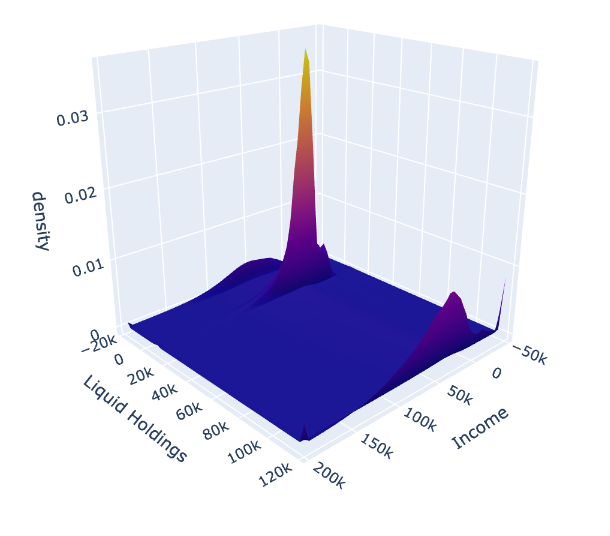
\includegraphics[width=0.8\linewidth]{Images/density.png}
    \caption{Empirical distribution function created using Statistics Netherlands microdata. Due to privacy legislation we have to use a cutoff point to prevent data about individuals to be deducable.}
    \label{fig:enter-label}
\end{figure}

\subsubsection{The general government}
The initial government debt, denoted as $L^{\mathrm{G}}_0$, is determined based on the consolidated gross debt (GD) of the Dutch government (sector S.13). This data is sourced from the Eurostat dataset on government deficit/surplus, debt, and associated metrics (gov\_10dd\_edpt1).

\subsubsection{The Bank} \label{sec:bank_initial_conditions}
The initial bank's equity, denoted as \(E_{k,0}\), is sourced from national accounting data, specifically the financial balance sheets (nasa{\_}10{\_}f{\_}bs), including F.5 and BF.90, which detail the non-consolidated equity and financial net worth of monetary financial institutions, excluding the central bank (S122\_S123). The initial bank's profits are calculated as the difference between initial income from interest and interest payments, represented by the equation:

\begin{equation*} 
	\textcolor{black}{\Pi_{k,0} = \mu \sum_{i} L_{i,0} + \bar{r}_{0} E_{k,0}},
 \end{equation*} 
where initial advances from the central bank, denoted as \(D_{k,0}\), are determined according to Equation \eqref{eq:bankreserves}.




\subsubsection{The Central Bank}
The initial central bank's equity, denoted as \(E^{\mathrm{CB}}_{0}\), is calculated as the residual on the central bank's liabilities. This is done by subtracting the initial bank reserves held (\(D_{k,0}\)) and the initial net creditor/debtor position with the rest of the world (\(D^{\mathrm{RoW}}_{0}\)) from the central bank's assets, which includes the initial government debt (\(L^{\mathrm{G}}_{0}\)). Consequently, the initial central bank's equity is defined according to Equation \eqref{eq:cbequity}. It is important to note that the initial balance of trade with the rest of the world (\(D^{\mathrm{RoW}}_{0}\)) is assumed to be zero, while the initial bank reserves held (\(D_{k,0}\)) are determined according to Equation \eqref{eq:bankreserves}.

